\section{复数}
\label{sec:ru-complex-numbers}

方程$x^2+1=0$在实数范围内没有解，因为实数的平方总不小于零。为了让这类方程也有解，引入一个新的数$i$，规定
\[
 i^2=-1,
\]
并允许它与实数一起按通常的规则相加、相乘。形如$z=a+bi$（$a,b\in\mathbb R$）的数称为\term{复数}（complex number），全体复数记作$\mathbb C$。
$a$称为$z$的实部，记作$\operatorname{Re}z$；$b$称为虚部，记作$\operatorname{Im}z$。两个复数相等，当且仅当实部、虚部分别相等。
$b=0$时$a+0i$就是实数$a$，所以$\mathbb R\subseteq\mathbb C$。下面先确定复数怎样运算，再给出它在平面上的表示。

\subsection{复数的四则运算}
\label{sec:ru-complex-arithmetic}

复数的加减按实部、虚部分别进行：
\[
 (a+bi)\pm(c+di)=(a\pm c)+(b\pm d)i.
\]
乘法先用分配律展开，再把$i^2$换成$-1$：
\[
 (a+bi)(c+di)=ac+adi+bci+bdi^2=(ac-bd)+(ad+bc)i.
\]
可以逐条验证，这样定义的加法与乘法仍满足交换律、结合律和分配律。

除法需要先把分母变成实数。称$\bar z=a-bi$为$z=a+bi$的\term{共轭复数}（complex conjugate），$|z|=\sqrt{a^2+b^2}$为$z$的\term{模}（modulus）。
由乘法公式，
\[
 z\bar z=(a+bi)(a-bi)=a^2+b^2=|z|^2,
\]
它是非负实数，并且只在$z=0$时为零。于是对$w\neq0$，把$z/w$的分子分母同乘$\bar w$，得到
\[
 \frac zw=\frac{z\bar w}{w\bar w}=\frac{z\bar w}{|w|^2}.
\]
右侧的分母是正实数，除法就化成了乘法和实数除法；条件$w\neq0$保证$|w|^2>0$。
共轭与运算相容：$\overline{z+w}=\bar z+\bar w$，$\overline{zw}=\bar z\,\bar w$，逐项展开即可验证。
由此$|zw|^2=zw\,\overline{zw}=(z\bar z)(w\bar w)=|z|^2|w|^2$，即$|zw|=|z|\,|w|$。

用一组具体的数核对这些关系。取$z=1+2i$、$w=3-i$，则$z+w=4+i$，
\[
 zw=3-i+6i-2i^2=5+5i.
\]
$|z|=\sqrt5$、$|w|=\sqrt{10}$，而$|zw|=\sqrt{50}=\sqrt5\cdot\sqrt{10}$，与模的乘法公式一致。除法为
\[
 \frac zw=\frac{(1+2i)(3+i)}{|3-i|^2}=\frac{3+i+6i+2i^2}{10}=\frac{1+7i}{10},
\]
回乘$w$可得$(3-i)(1+7i)/10=(10+20i)/10=1+2i$，结果正确。

复数虽然能做四则运算，却不能像实数那样比较大小。设复数上有一个全序$<$，并与运算相容：$x<y$蕴含$x+z<y+z$，$0<x$与$0<y$蕴含$0<xy$。
那么每个非零数的平方都为正：$x>0$时$x^2=x\cdot x>0$；$x<0$时两边加$-x$得$0<-x$，于是$x^2=(-x)^2>0$。
由此$1=1^2>0$，$-1=i^2>0$，两式相加得$0>0$，矛盾。所以后文的不等式总是比较实数，比如比较复数的模，而不比较复数本身。

\subsection{复数的几何意义}
\label{sec:ru-complex-geometry}

把$z=a+bi$对应到平面上的点$(a,b)$，就得到复数的平面表示，称为\term{复平面}（complex plane）：横轴表示实部，纵轴表示虚部。
由勾股定理，模$|z|=\sqrt{a^2+b^2}$是点$z$到原点的距离，$|z-w|$是两点之间的距离；加法按坐标相加，就是平面上的向量加法，共轭则是关于实轴的反射。
对$z\neq0$，从正实轴到射线$Oz$的转角$\theta$称为$z$的\term{辐角}（argument），它满足
\[
 a=|z|\cos\theta,\qquad b=|z|\sin\theta.
\]
转一整圈回到同一射线，所以辐角只确定到$2\pi$的整数倍：$\theta$与$\theta+2k\pi$（$k\in\mathbb Z$）表示同一个方向。
常取落在$(-\pi,\pi]$中的那个值，称为辐角主值。$z=0$位于原点，没有确定的方向，因而没有辐角。

记$r=|z|$，非零复数可以写成\term{三角形式}
\[
 z=r(\cos\theta+i\sin\theta).
\]
这一写法使乘法有了几何解释。设$z_1=r_1(\cos\theta_1+i\sin\theta_1)$，$z_2=r_2(\cos\theta_2+i\sin\theta_2)$，按乘法公式展开，再用三角函数的加法公式合并实部与虚部，得到
\[
 \begin{aligned}
 z_1z_2&=r_1r_2\bigl[(\cos\theta_1\cos\theta_2-\sin\theta_1\sin\theta_2)+i(\sin\theta_1\cos\theta_2+\cos\theta_1\sin\theta_2)\bigr]\\
 &=r_1r_2\bigl[\cos(\theta_1+\theta_2)+i\sin(\theta_1+\theta_2)\bigr].
 \end{aligned}
\]
所以乘以$z_2$，就是把点$z_1$到原点的距离乘以$r_2$，再绕原点逆时针转过$\theta_2$：模相乘，辐角相加。
例如$i=\cos(\pi/2)+i\sin(\pi/2)$，乘以$i$就是逆时针旋转直角，$i\cdot i=-1$正是把$1$转过两个直角。
图~\ref{fig:ru-complex-multiplication}(a)用前面的$z=1+2i$、$w=3-i$核对这一点。

\begin{figure}[!htbp]
 \centering
 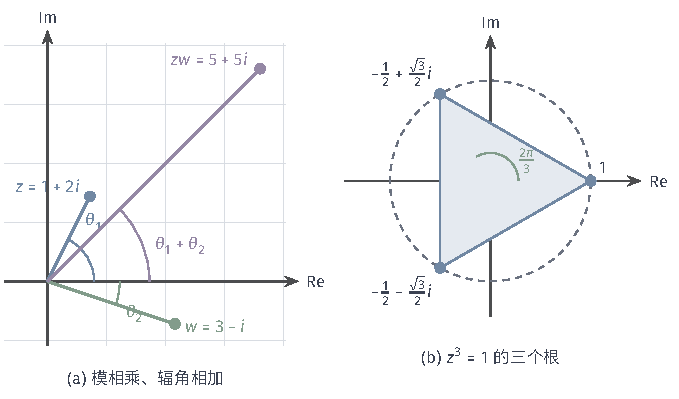
\includegraphics[width=112mm]{figures/01-mathematical-preliminaries-upper/02-real-numbers-and-univariate-functions/tikz/complex-multiplication-roots/figure.pdf}
 \caption{复数乘法与$n$次根的平面表示。(a)蓝、绿两点为$z=1+2i$与$w=3-i$，紫点为乘积$zw=5+5i$。乘积到原点的距离是$\sqrt5\cdot\sqrt{10}$，辐角是两个辐角之和，图中用弧线标出三个辐角。(b)$z^3=1$的三个根$1$与$-\tfrac12\pm\tfrac{\sqrt3}{2}i$都在单位圆上，辐角依次相差$2\pi/3$，构成正三角形的顶点。}
 \label{fig:ru-complex-multiplication}
\end{figure}

反复使用乘法公式并对$n$归纳，得到正整数次幂
\[
 z^n=r^n(\cos n\theta+i\sin n\theta).
\]
由$z\cdot r^{-1}(\cos(-\theta)+i\sin(-\theta))=1$，$z^{-1}$的模为$r^{-1}$、辐角为$-\theta$，所以公式对负整数次幂也成立。

反过来求$n$次根，就是找$w$使$w^n=z$。设$z=r(\cos\theta+i\sin\theta)$，$r>0$，$w=\rho(\cos\varphi+i\sin\varphi)$。
由幂公式，$w^n=z$要求$\rho^n=r$，并且$n\varphi$与$\theta$相差$2\pi$的整数倍。于是$\rho=r^{1/n}$，
\[
 \varphi=\frac{\theta+2k\pi}{n},\qquad k=0,1,\ldots,n-1.
\]
这$n$个辐角互不相差$2\pi$的整数倍，给出$n$个不同的根；$k$取其他整数时只是重复这些根。
它们到原点的距离相同，辐角依次相差$2\pi/n$，恰好是一个正$n$边形的顶点。
例如$z=1$时$r=1$、$\theta=0$，三次根为$1$与$\cos(2\pi/3)\pm i\sin(2\pi/3)=-\tfrac12\pm\tfrac{\sqrt3}2i$，如图~\ref{fig:ru-complex-multiplication}(b)。
三角形式中的$\cos\theta+i\sin\theta$还可以写成指数形式，那需要先用级数定义复指数，留到第~\ref{sec:ru-trig-expansion-complex-exponential}节。
